% Данный файл распространяетсяя под лицензией CC BY 4.0. Текст лицензии размещён на https://creativecommons.org/licenses/by/4.0/
% (c) Кафедра системного программирования, 2025

\documentclass[a4paper]{article}

\usepackage[a4paper, top=8mm, bottom=8mm, left=8mm, right=8mm]{geometry}

\usepackage{polyglossia}
\setdefaultlanguage[babelshorthands=true]{russian}
\setotherlanguage{english}

\usepackage{fontspec}
\setmainfont{FreeSerif}
\newfontfamily{\russianfonttt}[Scale=0.7]{DejaVuSansMono}

\usepackage[tiny, compact]{titlesec}

\usepackage{titling}
\setlength{\droptitle}{-1cm}
\pretitle{\begin{center}\begin{bfseries}\Large}
\posttitle{\par\end{bfseries}\end{center}}
\preauthor{\begin{center}\normalsize}
\postauthor{\par\end{center}\vspace{-1.8cm}}

\usepackage{hyperref}
\usepackage{bookmark}
\usepackage{csquotes}
\usepackage{graphicx}
\usepackage[table]{xcolor}
\usepackage{url}
\usepackage{float}

\title{Vortex: освоение FPGA-стека}

\author{Правкин Даниил Денисович}

\date{}

\begin{document}

\maketitle

\begin{flushright}
    Группа: \enquote{25.Б73-мм}

    Кафедра: Кафедра системного программирования


    Научный руководитель: Григорьев Семён Вячеславович

    
    Номер семестра практики: 2
\end{flushright} 


\section{Постановка задачи}

Vortex --- это проект с открытым исходным кодом, предназначенный для поддержки вычислений на графических процессорах (GPGPU). Он реализован на основе расширений системы команд RISC-V ISA и предусматривает возможность аппаратной конфигурации. Целью данной работы является получение навыков работы с FPGA-стеком.

Результаты работы необходимы для дальнейшей работы с Vortex: сборка Vortex, оценка потребления ресурсов конфигурации, сравнение различных конфигураций.

\section{Описание предлагаемого решения}

Vortex использует модель исполнения SIMT (Single Instruction Multiple Threads)\footnote{Информация из документации Vortex о микроархитектуре на сайте github.com (\url{https://github.com/vortexgpgpu/vortex/blob/master/docs/microarchitecture.md}) (27.04.2026)}, в рамках которой одна и та же инструкция выполняется над разными данными. Это достигается при помощи потоков (threads) --- наименьших единиц вычисления, выполняемых параллельно, --- и варпов (warps), которые представляют собой набор потоков, исполняющих одну и ту же инструкцию. За счёт этого достигается распараллеливание выполнения задачи. Одной из задач, выполняемой при помощи такой модели исполнения, является умножение матриц (например, в графических процессорах от компании NVIDIA)\footnote{В архитектуре CUDA, использующей SIMT, также есть функция умножения матриц (\url{https://docs.nvidia.com/cutlass/latest/media/docs/cpp/efficient_gemm.html}) (29.05.2026)}.

С целью получения навыков работы с Vortex был проведён эксперимент по измерению масштабируемости функции умножения матриц. Реализация решения осуществлялась в среде Docker-контейнера с применением симулятора SimX, поскольку он обеспечивает достаточно высокую потактовую точность, затрачивая при этом меньше времени на выполнение, чем RTL-симулятор.

\section{Эксперименты}

\subsection*{Цель}
Проанализировать масштабируемость функции умножения матриц при увеличении количества ядер и фиксированном объёме входных данных.

\subsection*{Входные данные}
Для эксперимента была выбрана матрица размера 512x512 с целью получения более реалистичной производительности. Для алгоритма требуется память для двух перемножаемых матриц и одной итоговой, следовательно, объём трёх матриц данного размера --- 3~МиБ, что превышает объём общей памяти (Local Memory) (128 КиБ), L1-кэша (16~КиБ), L2-кэша (1~МиБ) и L3-кэша (2~МиБ)\footnote{Объёмы общей памяти и l1/l2/l3-кэшей взяты со страниц Vortex на сайте github.com (объём общей памяти: \url{https://github.com/vortexgpgpu/vortex/blob/master/hw/rtl/mem/VX_local_mem.sv} оъёмы кэшей: \url{https://github.com/vortexgpgpu/vortex/blob/master/docs/simulation.md}) (26.04.2026)}; следовательно, программа будет больше взаимодействовать с основной памятью.

\subsection*{Проведение эксперимента}

Порядок выполнения тестов:
\begin{enumerate}
    \item Отключение графической оболочки, для повышения скорости симуляции.
    \item Запуск Docker-контейнера.
    \item Запуск тестов и запись результатов.
\end{enumerate}

Сперва надо было подобрать оптимальную конфигурацию для более реалистичной производительности. Подбор производился при cores=8, потому что большее количество ядер порождает большую нагрузку на память, то есть более реалистичную производительность.

Далее были выполнены тесты с оптимальной конфигурацией, но изменяемым количеством ядер. Значения количества ядер кратны степеням двойки, чтобы обеспечить более равномерное распределение нагрузки между ядрами, так как размер матрицы тоже кратен степени двойки.

\subsection*{Результаты и анализ}
В результате поиска аппаратной конфигурации (табл. \ref{tab:optimal_for_8}) наиболее оптимальной при восьми ядрах оказалась следующая: clusters=1, warps=8, threads=64, l2cache, l3cache.

По результатам тестов по измерению масштабируемости (рис. \ref{figure:sgemm_graph}), при увеличении числа ядер от 1 до 16 количество тактов уменьшается, а при cores=16 достигает наименьшего значения. В диапазоне от 17 до 31 в ходе экспериментов возникали ошибки, свидетельствовавшие о неудачной попытке разделить задачу между всеми вычислительными блоками. Например, при запуске конфигурации с 18~ядрами в итоговой статистике для двух из них были выведены отрицательные значения количества выполненных инструкций и затраченных тактов. При дальнейшем увеличении числа ядер (начиная с 32) наблюдался рост количества тактов. Это свидетельствует о накладных расходах, затрачиваемых на корректную работу вычислительных блоков, в том числе для обеспечения параллельного выполнения, вследствие чего суммарное количество превышает значение, полученное при 16 ядрах. Таким образом, для умножения матриц 512x512 при фиксированных параметрах (clusters=1, warps=8, threads=64, l2cache, l3cache) наименьшее количество тактов достигается при использовании 16 ядер.


\begin{table}
\centering
\begin{tabular}{| c|c|c |}
 \hline
 Кол-во групп потоков & Кол-во потоков & Кол-во тактов (млн.) \\
 \hline
 2 & 16 & 43,0 \\
 2 & 32 & 22,8 \\
 2 & 64 & 13,8 \\
 
 4 & 16 & 30,3 \\
 4 & 32 & 16,4 \\
 4 & 64 & 13,7 \\
 
 8 & 16 & 30,6 \\
 8 & 32 & 18,8 \\
 \rowcolor{lightgray}
 8 & 64 & 13,6 \\
 
 16 & 16 & 33,4 \\
 16 & 32 & 18,8 \\
 16 & 64 & 14,2 \\
 \hline
\end{tabular}
\caption{\label{tab:optimal_for_8} Число тактов, затраченных на выполнение алгоритма умножения матриц размера 512x512 при фиксированных параметрах (cores=8, clusters=1, l2cache, l3cache) и различных значениях числа потоков и групп потоков. Выделенная строка --- конфигурация, при которой затрачено наименьшее число тактов.}
\end{table}

\begin{figure}
    \centering
    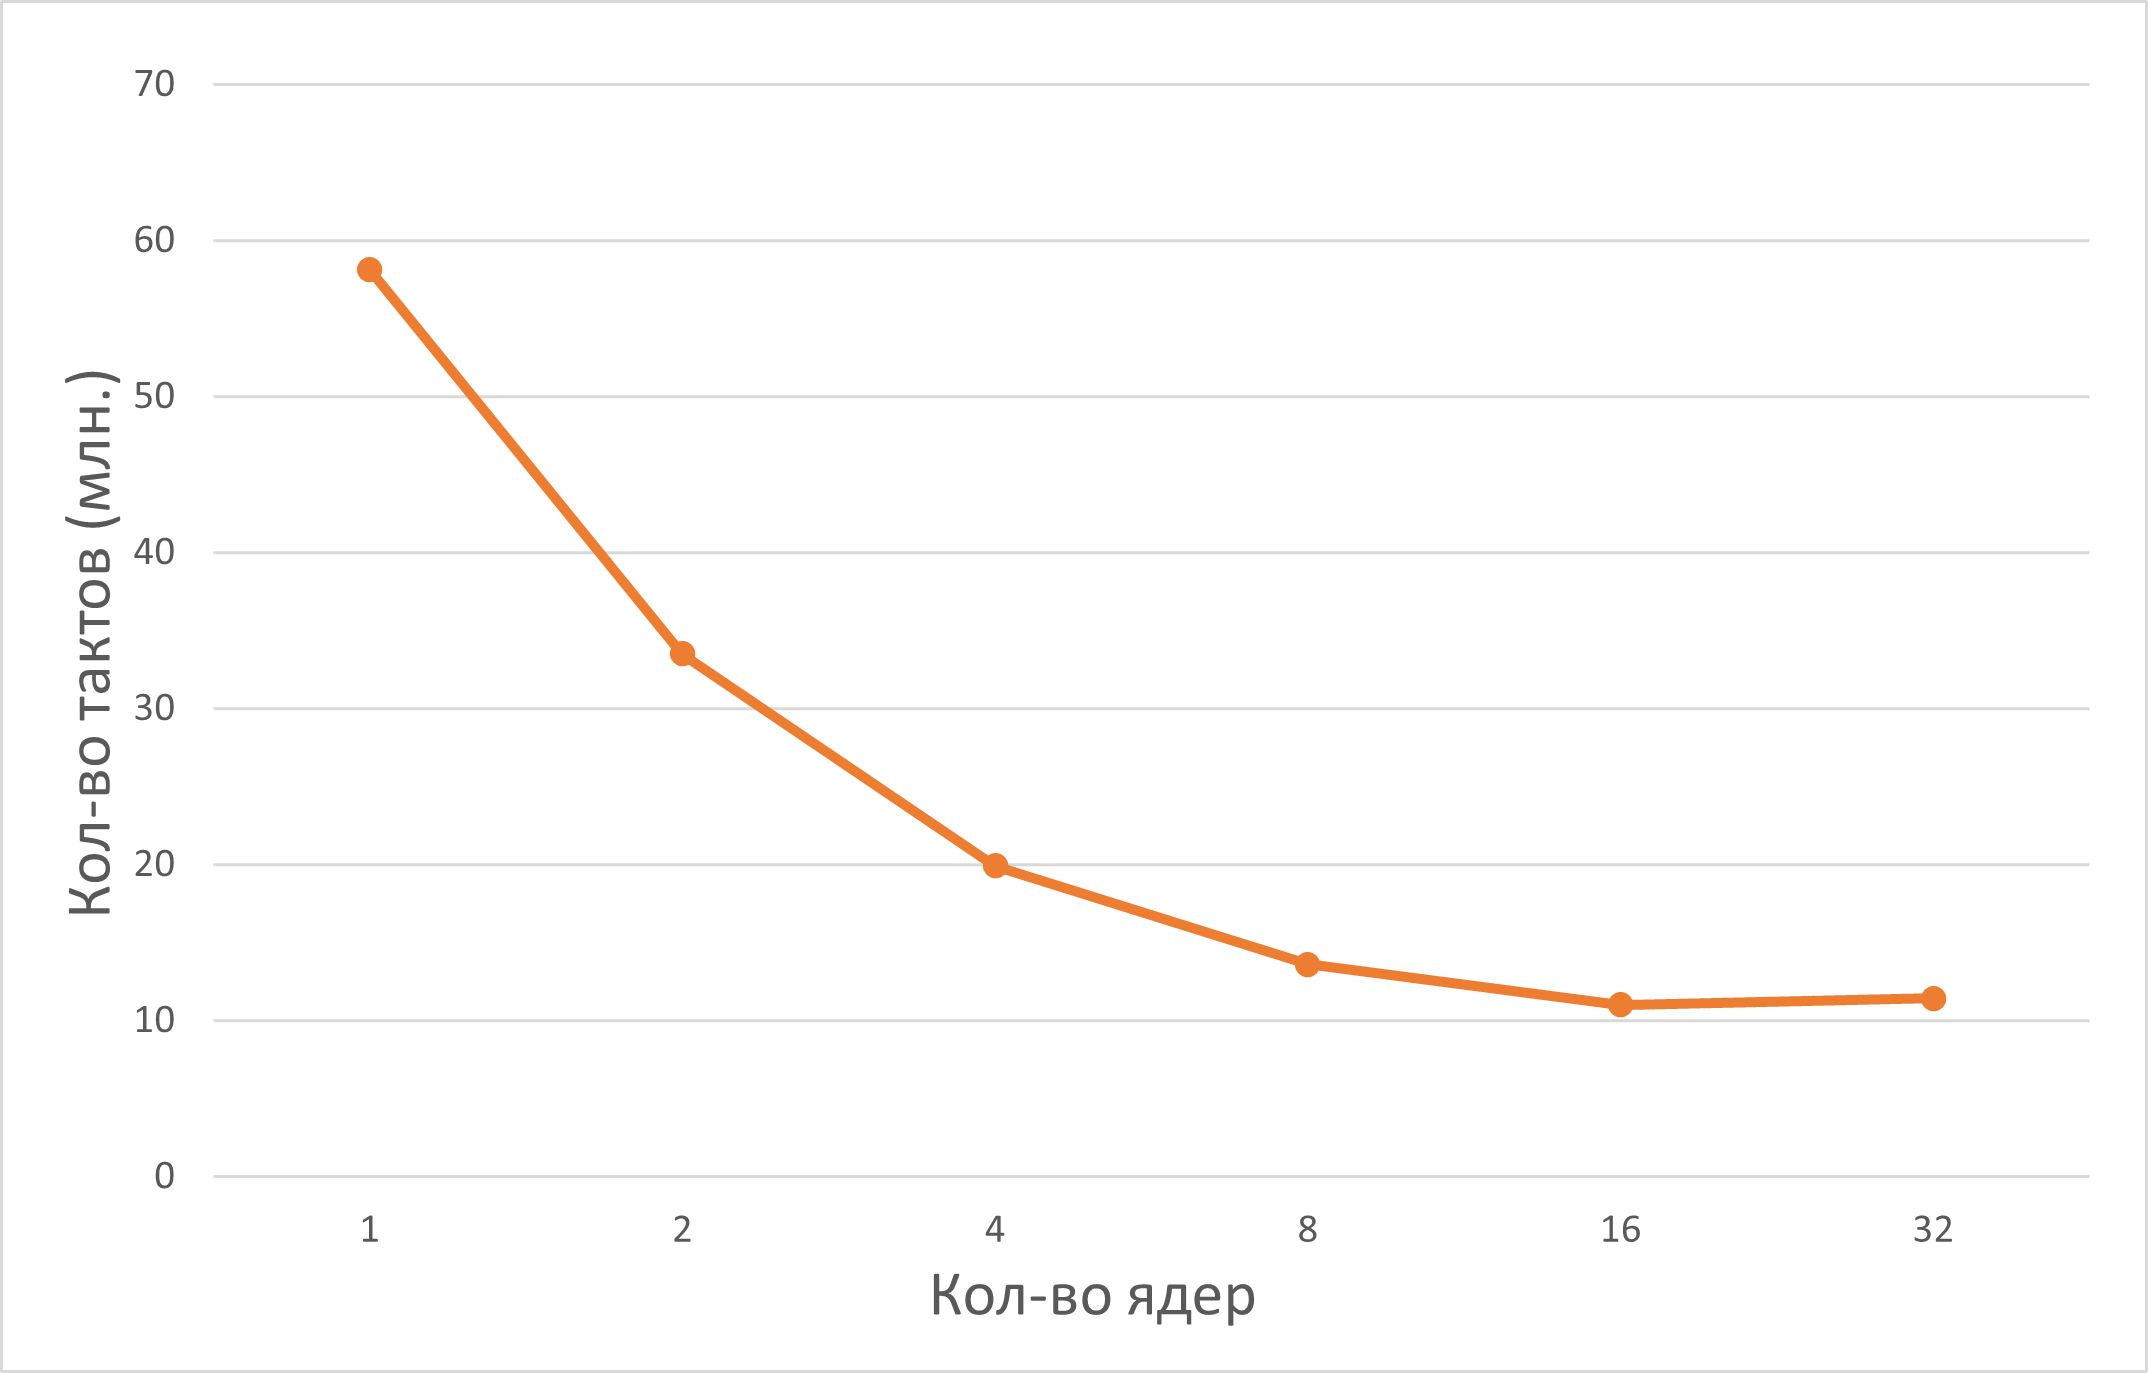
\includegraphics[width=0.8\linewidth]{sgemm_graph.png}
    \caption{\label{figure:sgemm_graph} Изменение числа тактов, затраченных на выполнение алгоритма умножения матриц при фиксированных параметрах (clusters=1, warps=8, threads=64, l2cache, l3cache) и различных значениях количества ядер.}
\end{figure}

\section{Заключение}

В ходе выполнения работы получены следующие результаты:

\begin{itemize}
    \item Произведено сравнение количества тактов, затрачиваемых различными конфигурациями Vortex при выполнении функции умножения матриц.
    \item Проанализирована масштабируемость функции умножения матриц.
\end{itemize}

Техническая документация: \url{https://github.com/Prosto-Dan/vortex_practice_1_year} .

\end{document}
